\documentclass[12pt]{article}
\usepackage[authoryear]{natbib}
\usepackage[english]{babel}
\usepackage{amsmath,amssymb}
\usepackage{graphicx}
\usepackage{amsthm}
\usepackage{epstopdf}
\usepackage{commath}
\usepackage{hyperref}
\usepackage{pstricks}
\usepackage{mathrsfs}
\usepackage{csquotes}
\usepackage{amssymb}
\usepackage{amsfonts}
\usepackage{mathtools}
\usepackage{makecell}
\usepackage{rotating}
\usepackage[font=small,labelfont=bf]{caption}
\usepackage{subcaption}
\usepackage{geometry}
\usepackage{setspace}
\usepackage{xr}
%\usepackage{bbm}
\usepackage{multirow}
\usepackage{enumitem}
%\usepackage[en-US]{datetime2}
\usepackage{color}
\usepackage{csvsimple,booktabs}
%\usepackage{booktabs} % For formal tables
\usepackage{fullpage}
%\usepackage[ruled,vlined]{algorithm2e}
\usepackage{algorithm}
\usepackage{algpseudocode}
\usepackage[stable]{footmisc}
\usepackage{pdfsync}

\newcommand{\E}{E}
%================================
% PATH

\graphicspath{{input/}{../../analysis/output/plot/}}

\newtheorem{theorem}{Theorem}
\newtheorem{fact}{Stylized Fact}
\newtheorem{corollary}{Corollary}[theorem]
\newtheorem{lemma}{Lemma}[section]
\newtheorem{proposition}{Proposition}
\theoremstyle{definition}
\newtheorem{defn}{Definition}
\newtheorem{step}{Step}
\newtheorem{remark}{Remark}[section]
\newtheorem{example-continued}{Example}
\newtheorem{example}{Example}
\newtheorem{assumption}{Assumption}
\newtheorem{cor}{Corollary}


\newcommand{\simon}[1]{\textcolor{olive}{\textbf{Simon: #1}}}
\newcommand{\chg}[1]{\textcolor{blue}{\textbf{#1}}}

\author{
        Simon Freyaldenhoven\\
        \textit{Federal Reserve Bank of Philadelphia\thanks{We thank XX for excellent research assistance. The views expressed herein are those of the authors and do not necessarily reflect the views of the Federal Reserve Bank of Philadelphia, or the Federal Reserve System. Emails: \href{mailto:simon.freyaldenhoven@phil.frb.org}{simon.freyaldenhoven@phil.frb.org}}}
}
\title{A quick note}


\date{\today}

\begin{document}

\maketitle

\begin{abstract}
\noindent This note illustrates how a draft uses the output produced by the code under \texttt{/analysis/}
\end{abstract}

JEL-Classification: C..

\textsc{Keywords}: TBA

\thispagestyle{empty}
% \newpage
% \tableofcontents
% \thispagestyle{empty}
\newpage

\setcounter{page}{1}

\section{The only section}

\begin{itemize}
\item We use bibtex for references (e.g. \cite{Freyaldenhoven2019}). 

\item Ideally all numbers should be softcoded, and come directly from output. For example, in our baseline simulations setup, where we simulate the throw of two 6-sided dice, the average sum of the two throws is equal to \input{../../analysis/output/estimation/baseline/mean_sum.txt}\unskip. That way all numbers are by construction always up-to-date.

\item Below, Figure \ref{fig:hist_baseline} includes a histogram of the simulation exercise.
\end{itemize}

\begin{figure}[tbh!]
\centering
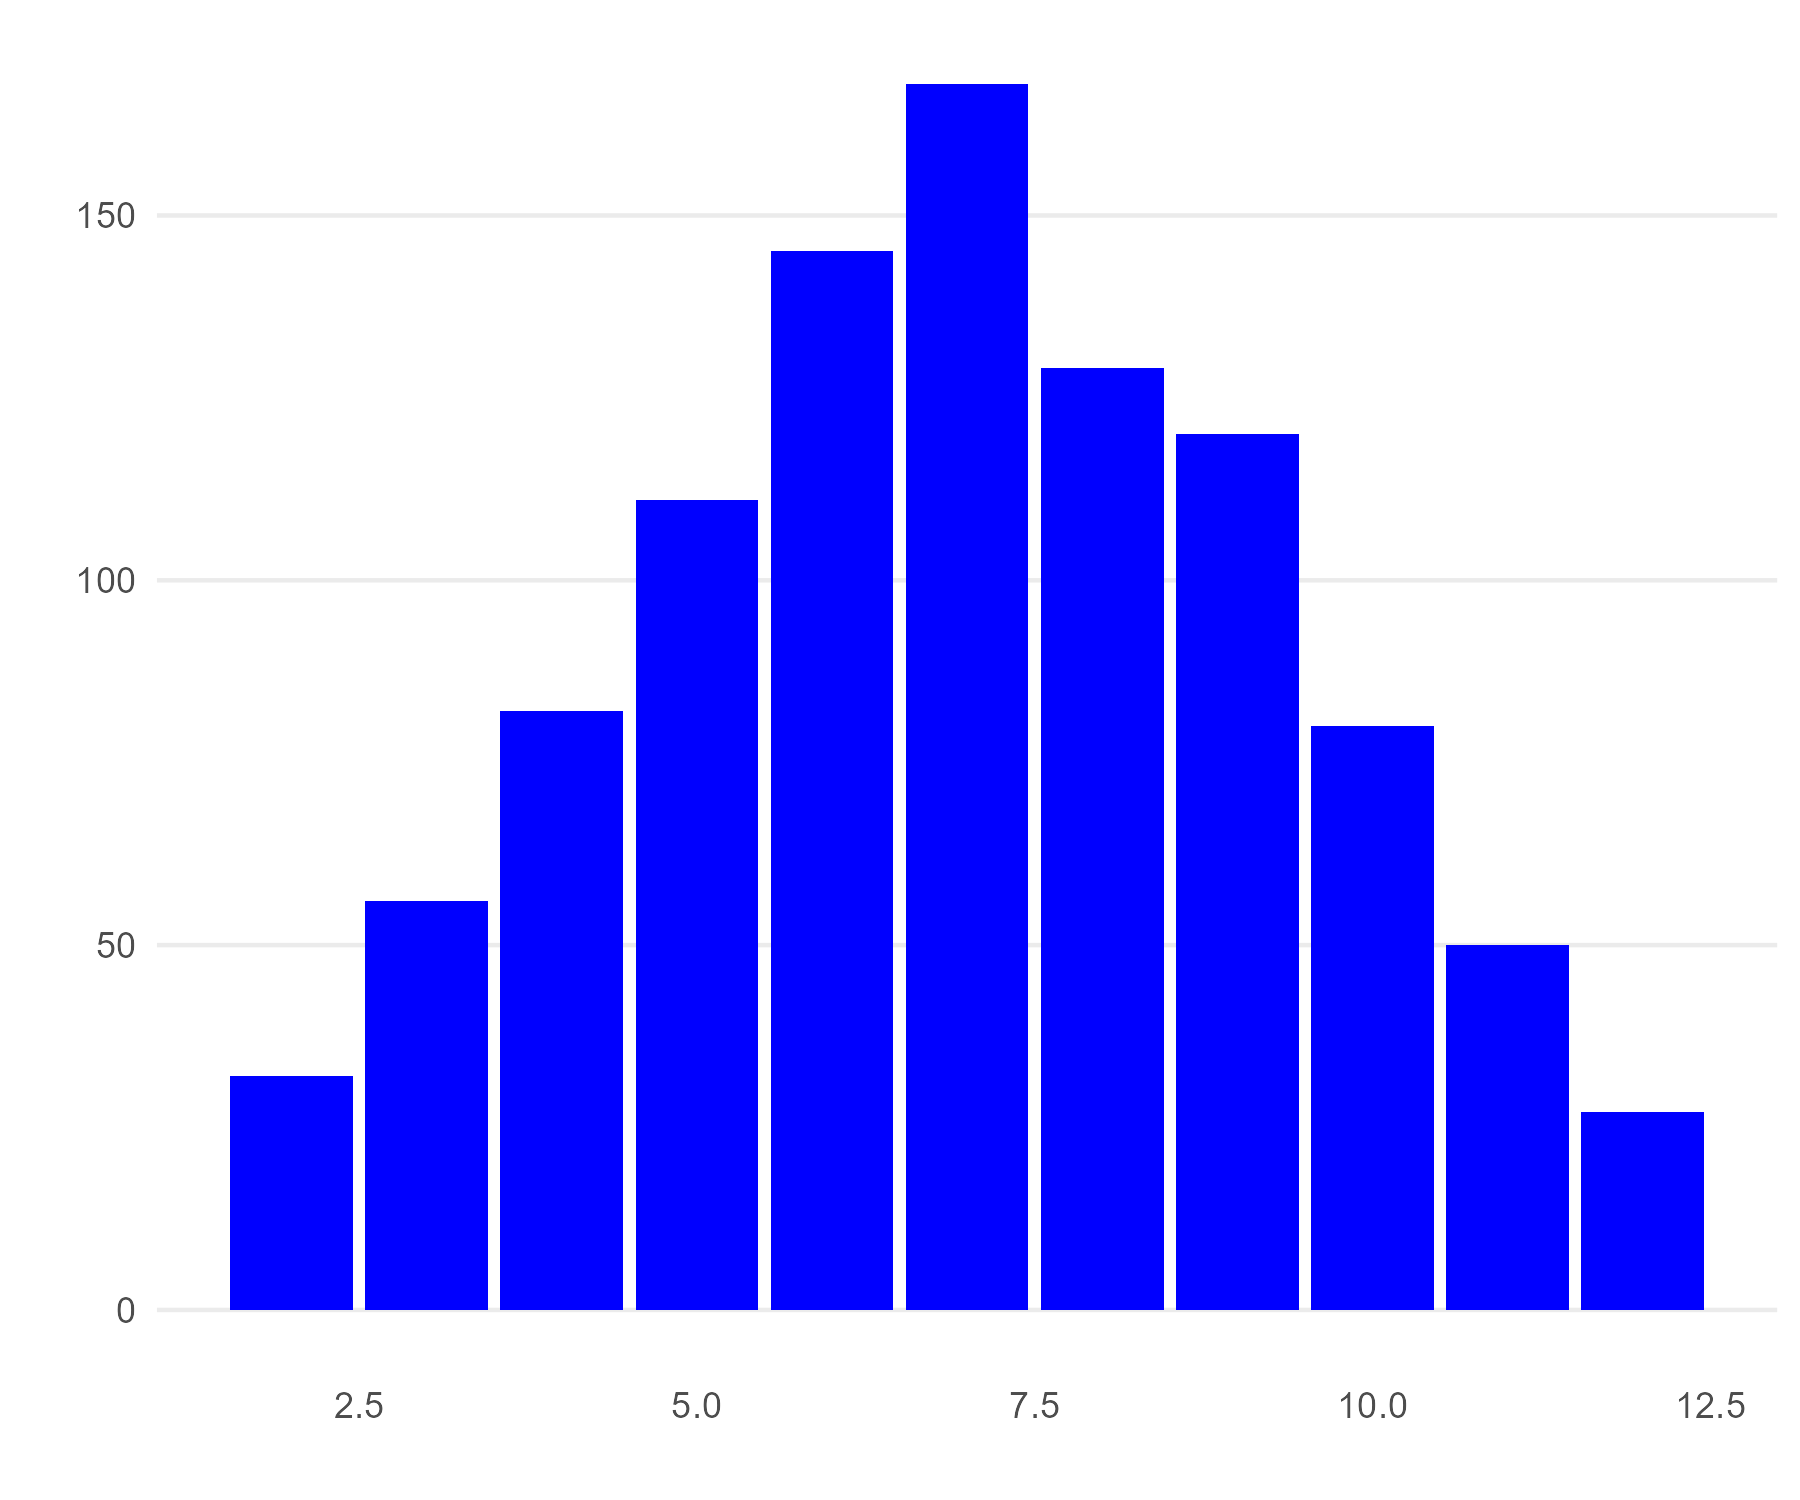
\includegraphics[width=.8\linewidth]{baseline/hist.png}
\caption[]{Numerical frequency for the sum of two six-sided die. Figure based on \input{../../analysis/output/estimation/baseline/sample_size.txt}throws.}
\label{fig:hist_baseline}
\end{figure}

%=======================================================
\bibliographystyle{plainnat}
\bibliography{example}
%\addbibresource{bib_fairness_mc}

%=======================================================

\end{document}


